\documentclass[t]{beamer}  % [t], [c], или [b] --- вертикальное выравнивание на слайдах (верх, центр, низ)
%\documentclass[handout]{beamer} % Раздаточный материал (на слайдах всё сразу)
%\documentclass[aspectratio=169]{beamer} % Соотношение сторон

%\usetheme{Berkeley} % Тема оформления
%\usetheme{Bergen}
%\usetheme{Szeged}

%\usecolortheme{beaver} % Цветовая схема
%\useinnertheme{circles}
%\useinnertheme{rectangles}

%\usetheme{HSE}

%%% Работа с русским языком
\usepackage{cmap}					% поиск в PDF
\usepackage{mathtext} 				% русские буквы в формулах
\usepackage[T2A]{fontenc}			% кодировка
\usepackage[utf8]{inputenc}			% кодировка исходного текста
\usepackage[english,russian]{babel}	% локализация и переносы

%% Beamer по-русски
\newtheorem{rtheorem}{Теорема}
\newtheorem{rproof}{Доказательство}
\newtheorem{rexample}{Пример}
\newtheorem{rproblem}{Задача}
\newtheorem{rsolve}{Решение}

%%% Дополнительная работа с математикой
\usepackage{amsmath,amsfonts,amssymb,amsthm,mathtools} % AMS
\usepackage{icomma} % "Умная" запятая: $0,2$ --- число, $0, 2$ --- перечисление

%% Номера формул
%\mathtoolsset{showonlyrefs=true} % Показывать номера только у тех формул, на которые есть \eqref{} в тексте.
%\usepackage{leqno} % Нумерация формул слева

%% Свои команды
\DeclareMathOperator{\sgn}{\mathop{sgn}}
\DeclareMathOperator{\card}{\mathop{card}} % Мощность множества
\DeclareMathOperator{\im}{\mathop{Im}} % Образ отображения
\DeclareMathOperator{\divergence}{\mathop{div}} % Дивергенция
\DeclareMathOperator{\rot}{\mathop{rot}} % Ротор

%% Перенос знаков в формулах (по Львовскому)
\newcommand*{\hm}[1]{#1\nobreak\discretionary{}
{\hbox{$\mathsurround=0pt #1$}}{}}

%%% Работа с картинками
\usepackage{graphicx}  % Для вставки рисунков
\graphicspath{{images/}{images2/}}  % папки с картинками
\setlength\fboxsep{3pt} % Отступ рамки \fbox{} от рисунка
\setlength\fboxrule{1pt} % Толщина линий рамки \fbox{}
\usepackage{wrapfig} % Обтекание рисунков текстом

%%% Работа с таблицами
\usepackage{array,tabularx,tabulary,booktabs} % Дополнительная работа с таблицами
\usepackage{longtable}  % Длинные таблицы
\usepackage{multirow} % Слияние строк в таблице

%%% Программирование
%\usepackage{etoolbox} % логические операторы

%%% Другие пакеты
\usepackage{lastpage} % Узнать, сколько всего страниц в документе.
\usepackage{soul} % Модификаторы начертания
\usepackage{csquotes} % Еще инструменты для ссылок
%\usepackage[style=authoryear,maxcitenames=2,backend=biber,sorting=nty]{biblatex}
\usepackage{multicol} % Несколько колонок

%%% Картинки
\usepackage{tikz} % Работа с графикой
\usepackage{pgfplots}
\usepackage{pgfplotstable}


\title{5 Неделя в \LaTeX}
\subtitle{Презентации \LaTeX}
\author{Константин Кравцов}
\date{3 июля 2020}
\institute[МФТИ]{Национальный исследовательский университет \\ <<МФТИ>>}

\begin{document}

\begin{frame}
	\maketitle
\end{frame}

\begin{frame}
	\frametitle{Уравнения Максвелла}
	Разбираемся с каждым уравнением
		\begin{itemize}
		\item $\displaystyle\divergence \textbf{D} = 4\pi\rho_{out}$
		\item $\displaystyle\rot \textbf{E} = - \frac{1}{c} \frac{\partial \textbf{B}}{\partial t}$
		\item $\displaystyle\divergence \textbf{B} = 0$
		\item $\displaystyle\rot \textbf{H} = \frac{4 \pi}{c} \textbf{j}_{out} + \frac{1}{c} \frac{\partial \textbf{D}}{\partial t}$
		\end{itemize}
\end{frame}

\begin{frame}
	\frametitle{Первое слагаемое: \ $\divergence \textbf{D} = 4\pi\rho_{out}$} % Попробовать без \displaystyle
		Это уже знакомая нам теорема Гаусса, который в интегральной форме выглядит следующим образом:\\
		\[
			\oint \left(\textbf{D}, d\textbf{S}\right) = 4\pi Q_{out}
		\]
		\begin{center}
		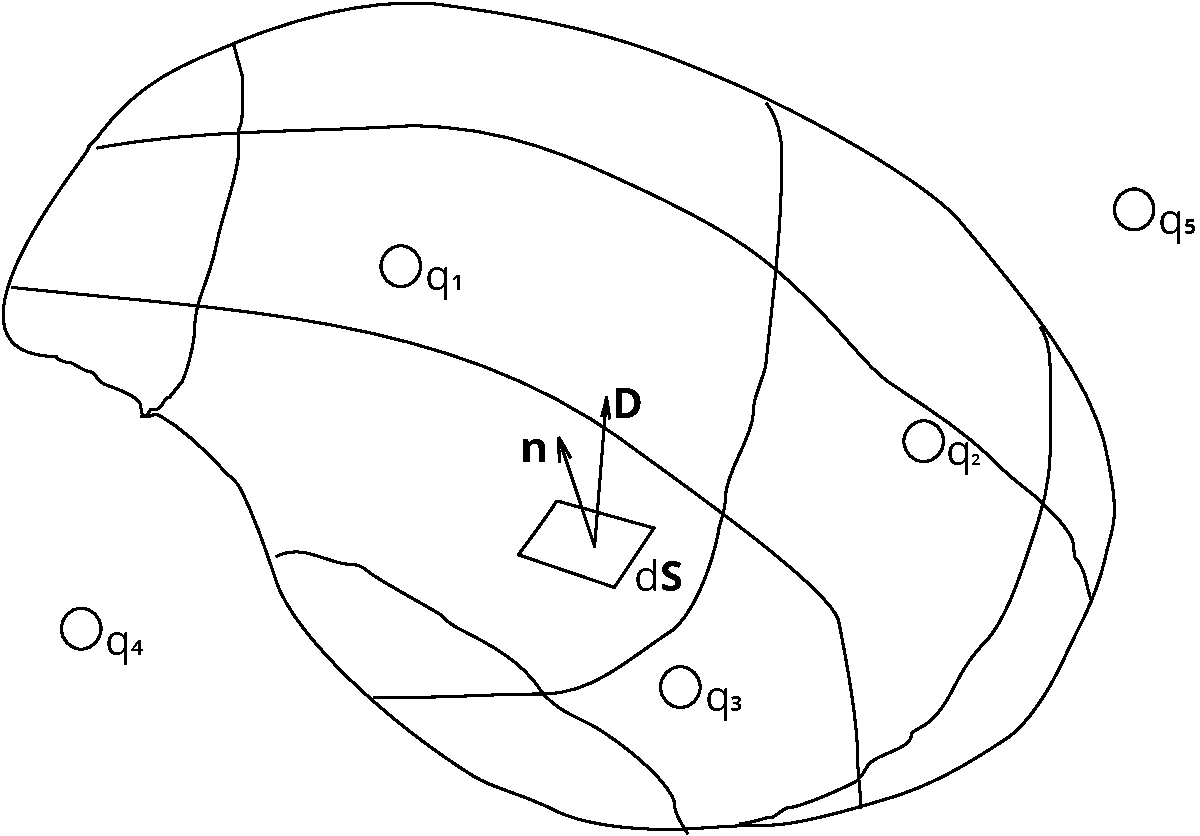
\includegraphics[scale=0.33333]{Thgauss}
		\end{center}
\end{frame}

\includeonlylecture{lec2}

\lecture{Занятие 1}{lec1}
	\section{Занятие 1}
	\begin{frame}
%		\title{jsagl} % Можно делать заголовки для каждой лекции
%		\maketitle
		\frametitle{\insertsection}
		Lecture number 1.	
	\end{frame}
	
\lecture{Занятие 2}{lec2}
	\section{Занятие 2}
	\begin{frame}
%		\title{jsagl} % Можно делать заголовки для каждой лекции
%		\maketitle
		\frametitle{\insertsection}
		Lecture number 2.	
		HEDM NOW!!!.
	\end{frame}

\begin{frame}
	\begin{rproblem}[HEDM]\label{HEDM}
		Текст задачи.
	\end{rproblem}
	\begin{rsolve}
		Текст решения задачи \ref{HEDM}.
	\end{rsolve}
\end{frame}

\end{document}